\documentclass{standalone}
\usepackage{fontspec}
\usepackage{sourcecodepro}
\usepackage{tikz}

\setmainfont{TeX Gyre Heros}
\setmonofont{Source Code Pro}

\usetikzlibrary{matrix, positioning, decorations.pathreplacing, calligraphy, fit, shapes}

\tikzset{
  dir/.style={draw=black, rounded corners=0.15cm, inner sep=0.5cm},
  file/.style={},
  boxlabel/.style={anchor=north east},
  fit label/.style={
    yshift={(height("#1")+8pt)/2},
    inner ysep={(height("#1")+16pt)/2},
    label={[anchor=north west]north west:#1}
  }
}

\begin{document}
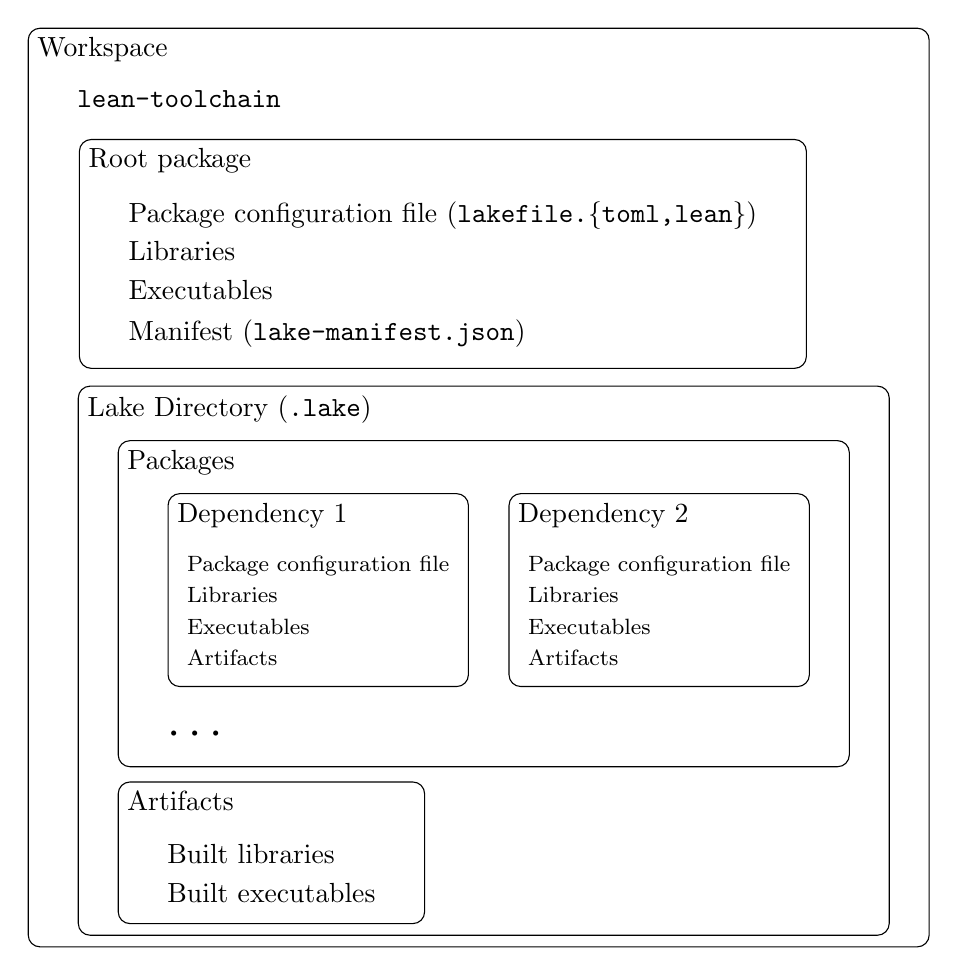
\begin{tikzpicture}[node distance=0.5cm]
\node[file](toolchain){\texttt{lean-toolchain}};

\begin{scope}[node distance=0.5cm]
\node[file,below=1.25cm of toolchain.south west, anchor=west, xshift=0.65cm](lakefile){Package configuration file (\texttt{lakefile.\{toml,lean\}})};
\node[below=of lakefile.north west, anchor=north west](lib){Libraries};
\node[below=of lib.north west, anchor=north west](exe){Executables};
\node[below=of exe.north west, anchor=north west](manifest){Manifest (\texttt{lake-manifest.json})};
\node[dir, fit=(lakefile)(lib)(exe)(manifest), fit label={Root package}](src){};
\end{scope}

\begin{scope}[node distance=0.4cm, dir/.style={draw, font=\footnotesize, rounded corners=0.15cm}, file/.style={font=\footnotesize}]]
\node[file,below=2.25cm of src.south west, anchor=north west, xshift=1.25cm](lakefile1){Package configuration file};
\node[file, below=of lakefile1.north west, anchor=north west](lib1){Libraries};
\node[file, below=of lib1.north west, anchor=north west](exe1){Executables};
\node[file, below=of exe1.north west, anchor=north west](art1){Artifacts};
\node[dir, fit=(lakefile1)(lib1)(exe1)(art1), fit label={Dependency 1}](dep1){};
\end{scope}

\begin{scope}[node distance=0.4cm, dir/.style={draw, font=\footnotesize, rounded corners=0.15cm}, file/.style={font=\footnotesize}]]
\node[file,right=0.75cm of lakefile1.north east, anchor=north west](lakefile2){Package configuration file};
\node[file, below=of lakefile2.north west, anchor=north west](lib2){Libraries};
\node[file, below=of lib2.north west, anchor=north west](exe2){Executables};
\node[file, below=of exe2.north west, anchor=north west](art2){Artifacts};
\node[dir, fit=(lakefile2)(lib2)(exe2)(art2), fit label={Dependency 2}](dep2){};
\end{scope}

\node[file,below=of art1.south west, anchor=north west, xshift=-0.25cm](morepackages){\LARGE $\cdots$};

\node[dir, fit=(dep1)(dep2)(morepackages), fit label={Packages}](pkgs){};


\begin{scope}[node distance=0.5cm]
  \node[file, below=1cm of morepackages.south west, anchor=north west](builtlib){Built libraries};
  \node[file, below=of builtlib.north west, anchor=north west](builtexe){Built executables};
\end{scope}
\node[dir, fit=(builtlib)(builtexe), fit label={Artifacts}](arts){};

\node[dir, fit=(pkgs)(arts), fit label={Lake Directory (\texttt{.lake})}](builddir){};


\node[dir, fit=(src)(lakefile)(toolchain)(builddir), fit label={Workspace}](ws){};
\end{tikzpicture}
\end{document}

% Local Variables:
% TeX-engine: luatex
% End:
